\chapter{PlayStation}

V roce 1995 se společnost \textit{Sony Computer Entertainment} rozhodla vydat herní konzoli \textit{PlayStation}. 
Toto rozhodnutí bylo reakcí na rozpadlý vztah s firmou \textit{Nintendo}, se kterou měla \textit{Sony} spolupracovat na vytvoření nové herní konzole, jak můžeme vidět v obrázku \ref{sony-and-nintendo-console}, 
umožňující využívání jak \textit{CD}, tak i kazet jako úložné médium. 
Díky ambicím ze strany \textit{Sony} a nepřátelství vůči \textit{Nintendu} se \textit{PlayStation} konzole odlišovala v mnoha ohledech od svých konkurentů, 
a právě tyto změny vyvolaly významný ohlas a zajistily této konzoli úspěch, viz obrázek \ref{psx-console}.

V současné době je \textit{PlayStation} šestou nejlépe prodávanou herní konzolí\footnote{Seznam nejlépe prodávaných videoherních konzolí: \url{https://en.wikipedia.org/wiki/List_of_best-selling_game_consoles}}, čímž se stala velmi populárním systémem. 
Konzole obsahovala následující hardware\footnote{Technická specifikace PlayStation konzole: \newline \url{https://en.wikipedia.org/wiki/PlayStation_technical_specifications}}:

\begin{itemize}
    \label{Specifikace Hardwaru}
    \item{\textbf{CPU} - MIPS R3000A 33.8688MHz}
    \item{\textbf{RAM} - 2MiB EDO DRAM}
    \item{\textbf{Geometry Transformation Engine (GTE)} - Akcelerátor lineární algebry}
    \item{\textbf{Motion Decoder (MDEC)} - Dekodér JPEG obrázků}
    \item{\textbf{GPU} - 32bit Sony GPU, 1MB VRAM}
    \item{\textbf{SPU} - 16bit Sony SPU}
    \item{\textbf{CD-ROM}}
\end{itemize}

\begin{figure}[hbt]
	\centering
	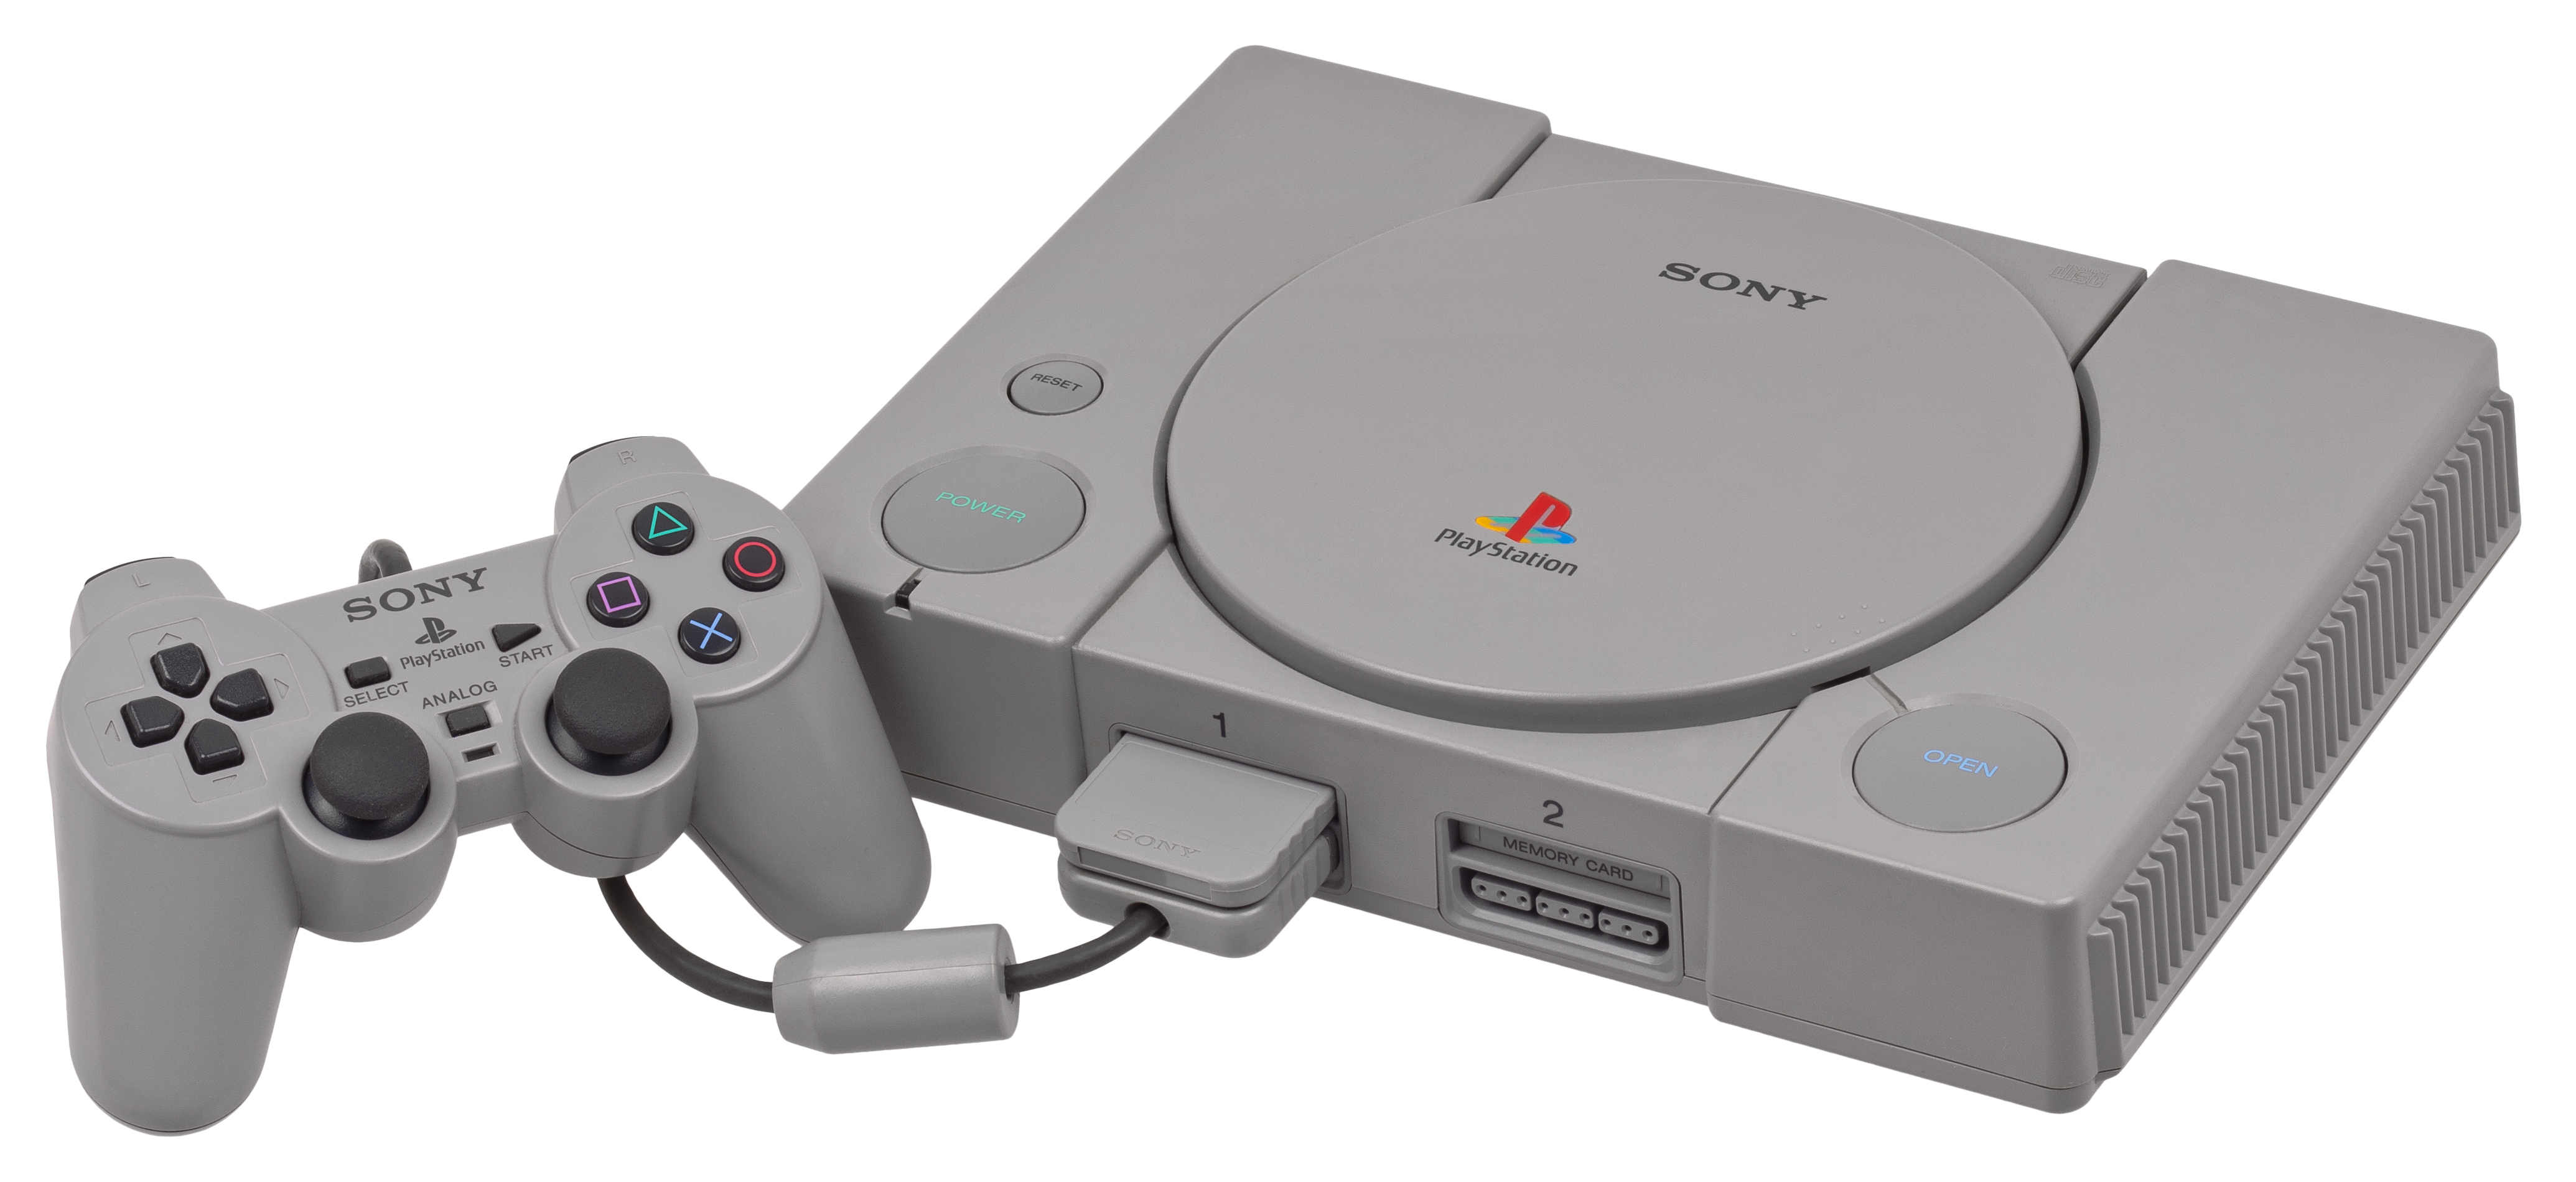
\includegraphics[width=0.7\textwidth]{obrazky-figures/psx-console.jpg}
	\caption[Úspěch \textit{PlayStation 1}]{První pokus společnosti \textit{Sony} proniknout na herní trh byl velmi úspěšný. Celkem se prodalo přibližně 102,49 milionu kusů. Pro srovnání, \textit{Nintendo 64} od společnosti \textit{Nintendo} se prodalo pouze 32,93 milionu}
	\label{psx-console}
\end{figure}

\begin{figure}[hbt]
	\centering
	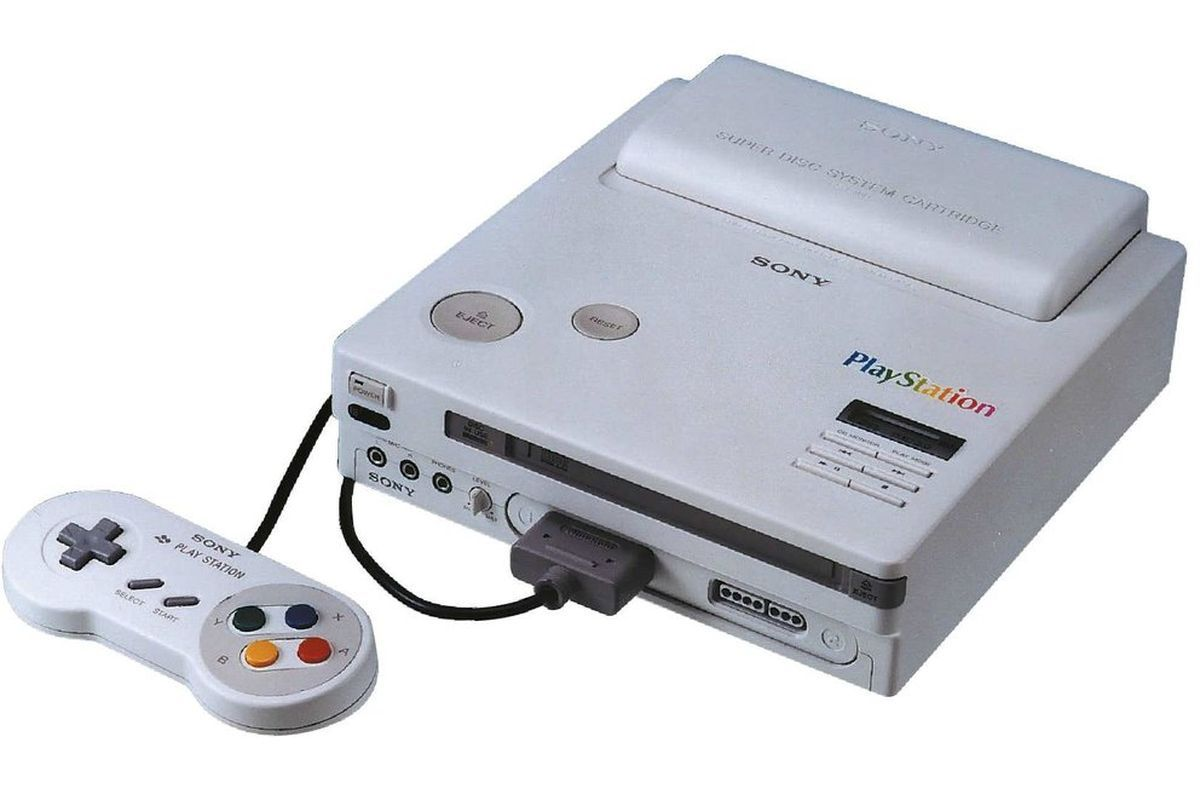
\includegraphics[width=0.7\textwidth]{obrazky-figures/sony-and-nintendo-console.jpg}
	\caption[\textit{Nintendo PlayStation}]{Nedávno se objevil prototyp konzole, která je důkazem vztahu mezi společnostmi \textit{Sony} a \textit{Nintendo}. Konzole fungovala jako hybrid, do kterého bylo možné nahrávat hry z \textit{CD} nebo kazet. Nakonec tato konzole nebyla nikdy vydána, protože \textit{Sony} chtělo kontrolovat licencování \textit{CD} verzí her a \textit{Nintendo} to tento požadavek zamítlo \cite{PlayStationNintendo}.}
	\label{sony-and-nintendo-console}
\end{figure}

\section{NTSC/PAL a bezpečnost}

V roce \textit{1995} byla hlavní televizní technologií stále \textit{Cathode Ray Tube (CRT)}, přičemž existovaly dva standardy, které specifikovaly enkódování a zobrazování barev na těchto analogových zařízeních. 
Tyto standardy byly pojmenovány \textbf{NTSC} a \textbf{PAL} přičemž to, s jakým standardem se člověk mohl setkat, záviselo na jeho geografické poloze. 
\textit{PlayStation} konzole samozřejmě musela s těmito rozdíly počítat a rozlišovala celkem tři různé regiony:\\[\baselineskip]

\begin{minipage}{\textwidth}
\begin{itemize}
    \item{\textbf{USA} - NTSC}
    \item{\textbf{Japonsko} - PAL}
    \item{\textbf{Evropa} - PAL}
\end{itemize}
\end{minipage}
\\[\baselineskip]

Tyto dva standardy definovaly vertikální rozlišení, 
snímkovou frekvenci a také verzi \textit{BIOSu}, který konzole obsahovala\footnote{NTSC/PAL rozdíly \cite{PSXSpec}: \url{https://psx-spx.consoledev.net/graphicsprocessingunitgpu/\#vertical-video-timings}}. 
Aby se \textit{Sony} vyhnulo licenčním problémům a předešlo pirátství, regionálně uzavřelo každou konzoli tak, že každá konzole měla ve svém \textit{BIOSu} regionální podpis. 
Poté na každém \textit{CD} obsahujícím hru byla vypálena jedna ze tří regionálních značek. 
Tento speciální segment se nacházel velmi blízko středového otvoru \textit{CD} a 
konvenční \textit{CD-ROM} čtečky nebyly schopné tento region číst ani do něj cokoliv vypalovat.

Při bootování hry byl tento speciální segment přečten a porovnán s regionálním kódem \textit{BIOSu}, 
a pokud se tyto podpisy neshodovaly, konzole odmítla hru načíst.

Tento způsob ochrany byl velmi prostý, ale účinný. Speciální vypalovače vlastnila pouze \textit{Sony}, 
a tedy oficiálně licencované \textit{CD} disky nebylo možné zreplikovat. 
Nicméně tato forma ochrany nebyla perfektní a relativně brzy byly objeveny způsoby, jak tento systém obejít.

Prvním způsobem bylo vytvoření hardwarového čipu, který člověk nainstaloval do konzole\footnote{Stealth chip: \url{https://www.r43ds.org/products/PS1-Modchip-Playstation-Stealth-Mod-chip.html}}. 
Tento čip pak figuroval jako prostředník mezi \textit{CD-ROM} a \textit{BIOSem}
a kdykoliv byl speciální region kód \textit{BIOSem} vyžádán, čip zaslal falešná data s nimiž byl \textit{BIOS} spokojen.
Nicméně jisté hry, jako například \textit{Spyro 2}, dokázaly detekovat prezenci tohoto čipu a znemožnit hráči v postupu ve hře,
nebo mu tento postup potají zásadně znepříjemnily. Toto vítězství na straně \textit{Sony} však mělo krátkou životnost, jelikož
vývojáři čipu vytvořili tzv.: \textit{Stealth mod-chip}, který se po zaslání falešných informací uměl deaktivovat.

Druhým způsobem obejití ochrany byla technika nazvaná \textit{Disc Swapping}.
Tento exploit byl založen na faktu, že \textit{CD-ROM} mechanika používala fyzický spínač, 
pomocí kterého detekovala, zda je poklop zavřen či otevřen. 
Uživatel mohl tento spínač, například pomocí kusu plastu nebo složeného papíru, uměle ovládat a donutit tak \textit{CD-ROM} mechaniku si myslet, že poklop je uzavřen. 
Uzavření poklopu byl signál pro konzoli, aby začala načítat hru a provést kontrolu regionálního kódu. 
Jakmile kontrola byla provedena, uživatel se stále otevřeným poklopem oficiální \textit{CD} rychle vyměnil za neoficiální \textit{CD}, 
a tím byl exploit hotov. Konzole si pak myslela, že obsahuje legitimní \textit{CD}, což ale nebyla pravda.

Konečné naložení s piráctvím pak \textit{Sony} řešilo na softwarové úrovni tak, že do \textit{sub-kanálů}\footnote{CD-ROM subchannels: \url{https://en.wikipedia.org/wiki/Compact_Disc_subcode}} disku zapisovala speciální
klíče, které tehdejší běžné \textit{CD-ROM} mechaniky nedokázaly replikovat. Poté za běhu hra spustila několik kryptografických kontrol, jako například
\textit{CRC} kontrolní sumu nad svými daty, přičemž pokud na disku chyběly \textit{sub-kanály} s klíči, hra poté stejně jako v předchozích situacích
odmítla hru spustit, nebo například v případě hry \textit{Spyro 3}, hra hráči dovolila pokračovat do určitého bodu a pak mu bez
varování smazala uložený postup na paměťové kartě. V tomto případě hry musely být individuálně analyzovány a pro každou hru bylo
nutné vytvořit záplaty pro vypnutí těchto kontrol, aby hra byla spustitelná na zkopírovaném disku.

\section{Existující emulátory}

Popularita této konzole je samozřejmě patrná z mnoha hledisek. 
Nejenže v roce 2020 \textit{Sony} vydalo pátou generaci své herní konzole, 
ale dodnes existuje dedikovaná komunita nadšenců, kteří tuto konzoli dokázali rozebrat do posledního šroubku \cite{PSXSpec}. 
Existují rozsáhlé dokumenty, které popisují tuto konzoli do každého detailu, a díky tomu existuje celá řada emulátorů. 
To, co také činí tento systém populárním v těchto kruzích je, že na tehdejší dobu tato konzole měla z velké části modularní design. 
Herní systémy té a předchozí doby měly mnoho komponent, které byly doslova \textit{natvrdo zadrátovány} a neposkytovaly žádnou flexibilitu. 
I přesto, že \textit{PlayStation} do této kategorie hardwarového designu částečně spadá, celý systém je navržen spíše jako moderní stolní počítač.

V dnešní době emulátory nejen poskytují velmi přesnou emulaci \textit{PlayStation} systému, 
ale také nabízejí nespočet vylepšení oproti původnímu systému, které zpříjemňují jeho použití.
Například emulátor \textit{DuckStation}\footnote{Duckstation github repozitář: \url{https://github.com/stenzek/duckstation}} umožňuje uložit současný stav celé konzole (\textit{Save State}) 
a vytvořit tak snímek v čase, který člověk může později obnovit. 
Tato vlastnost se hodí v obtížných videohrách, ve kterých se ukládá postup zřídka, 
a tedy umožňuje hráči si diktovat uložení postupu dle vlastního uvážení.

Další vymožeností, kterou disponuje emulátor \textit{PCSX ReARMed}\footnote{PCSX ReARMed github repozitář: \url{https://github.com/notaz/pcsx_rearmed}}, 
je vlastní implementace \textit{High-Level Emulation (HLE)} \textit{BIOSu}. 
\textit{BIOS} je nedílnou součástí každé \textit{PlayStation} konzole. Stará se jednak o inicializaci hardwaru, 
ale také figuruje jako velmi jednoduchý operační systém, který videohry, stavěné na tomto systému, 
mohou používat pro usnadněný přístup k hardwaru. Tento fakt nutí každého uživatele emulátoru 
\textit{BIOS} extrahovat z původní konzole nebo jej získat nelegálními prostředky. 
Emulátor \textit{PCSX ReARMed} se pokusil celý \textit{BIOS} dekompilovat a implementovat ho přímo do vlastního systému.

Většina emulátorů také nabízí možnost \textit{Just-in-Time (JIT)} kompilace \textit{PlayStation} 
procesoru buď na \textit{x86\_64} či \textit{arm} architekturu. Transformace instrukcí \textit{PlayStation} 
procesoru na nativní procesor za běhu má za následek velké zisky v oblasti výkonu. Emulátor \textit{PCSX ReARMed} 
jde ještě dál a určité hardwarové komponenty \textit{PlayStation} systému implementuje pomocí ručně 
psaného \textit{arm assembly} kódu, což umožňuje získat nemálo výkonu zejména u mobilních zařízení, u kterých dominuje \textit{arm} architektura.

Velmi impozantním projektem je také \textit{MiSTer FPGA PSX}\footnote{MiSTer FPGE PSX github repozitář: \url{https://github.com/MiSTer-devel/PSX_MiSTer}}, 
což je práce snažící se implementovat \textit{PlayStation} emulátor na \textit{FPGA} čipu.

\section{Renderovací rozlišení}

\begin{figure}[hbt]
    \centering
    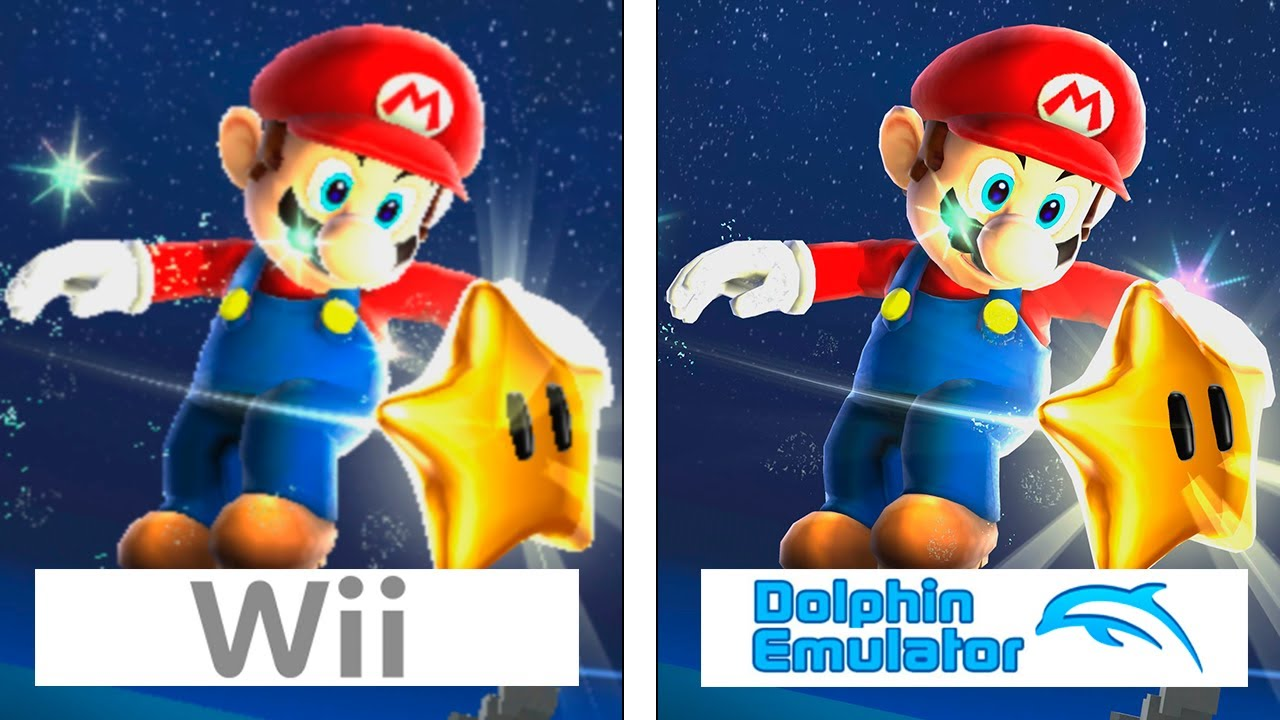
\includegraphics[width=0.8\textwidth]{obrazky-figures/dolphin-resolution.jpg}
    \caption[Příklad zvýšení rozlišení]{\textit{Dolphin} emulátor umí zvýšit interní renderovací rozlišení, což může vylepšit herní zážitek}
    \label{dolphin-resolution}
\end{figure}

Nepochybně je ekosystém okolo konzole \textit{PlayStation} velmi vyzrálý. 
Mít možnost si bez větších problémů užít videohry z 90. let je velmi uspokojivé z hlediska zachování videoherní historie. 
Přestože existuje několik vyspělých emulátorů s mnoha vychytávkami, 
žádný z nich se nesoustředí na vylepšení grafické prezentace, jako například možnost 
změnit velikost interního renderovacího rozlišení\footnote{Ukázka změny rozlišení: \url{https://www.youtube.com/watch?v=LSIYalc1D6Y}}, viz obrázek \ref{dolphin-resolution}. Tento nápad není originální a lze ho nalézt v emulátorech různých konzolí jako jsou například:

\begin{itemize}
\item{\textbf{Citra} - emulátor \textit{Nintendo 3DS}\footnote{Citra github repozitář: \url{https://web.archive.org/web/20240304191755/https://github.com/citra-emu/citra}}}
\item{\textbf{Dolphin} - emulátor \textit{Nintendo Gamecube/Wii}\footnote{Dolphin github repozitář: \url{https://github.com/dolphin-emu/dolphin}}}
\item{\textbf{PCSX2} - emulátor \textit{Sony PlayStation 2}\footnote{PCSX2 github repozitář: \url{https://github.com/PCSX2/pcsx2}}}
\end{itemize}

Tato schopnost emulátoru je možná díky tomu, že systémy jako \textit{Nintendo Gamecube} 
či \textit{PlayStation 2} mají podobnou grafickou pipeline jako moderní systémy, 
a tedy není tak složité modifikovat emulátor tak, aby vykresloval do většího prostoru. \textit{PlayStation} má velmi netradiční zpracování 
grafiky (např.: chybějící \textit{z-buffer}, žádná perspektivní korekce, ...) a vykreslování ve vyšším 
rozlišení je tedy složitější, protože nemálo her na těchto netradičních hardwarových funkcích napevno závisí.
Tato práce se tedy nezabývá pouze implementací emulátoru, ale také zvyšováním renderovacího rozlišení \textit{GPU} komponenty systému.
